\section{appendix}

This section explains more in depth the different choices and assumptions that were made during the creation of the different models as well as explaining the equations within them.


\subsection{Dashboard screenshots}
\begin{figure*}[!htb]
    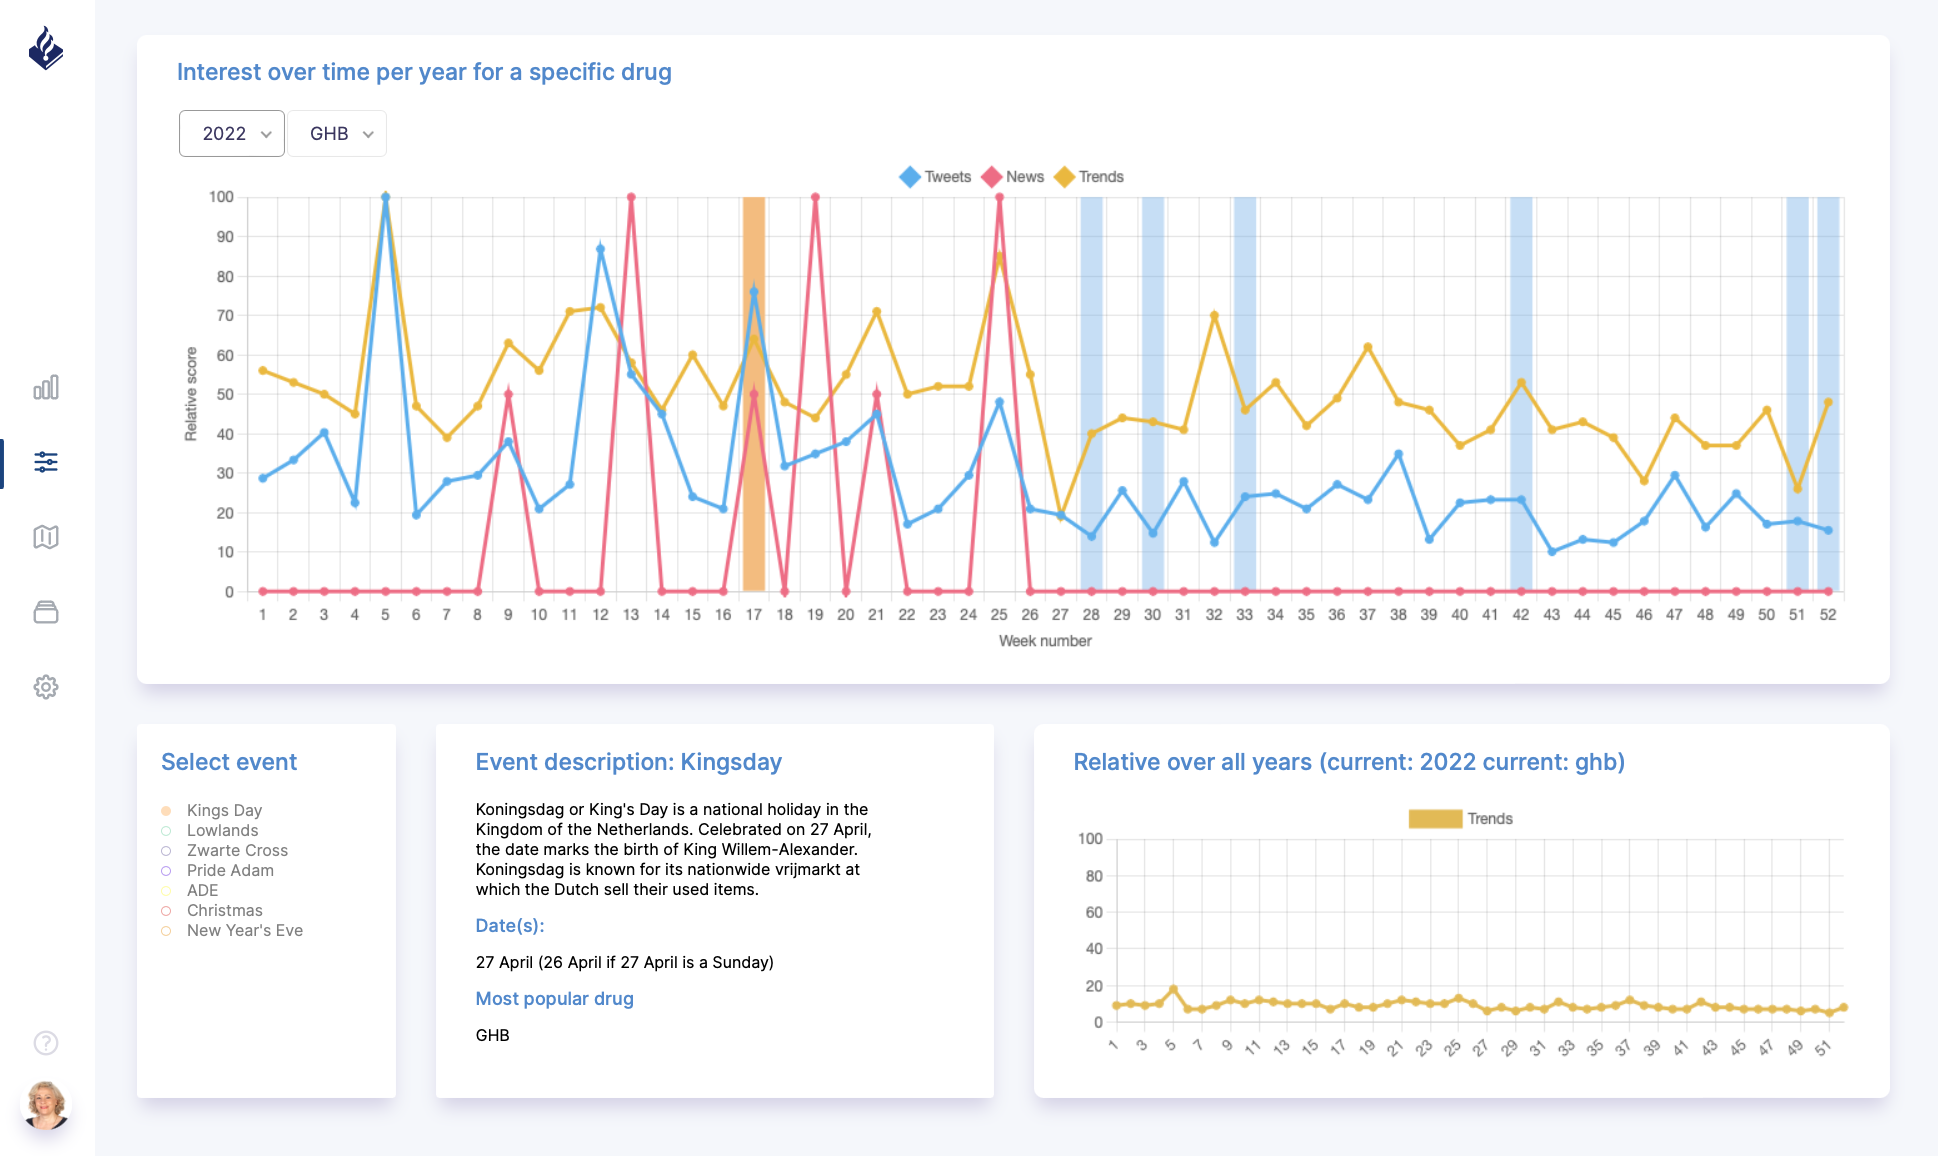
\includegraphics[width=\textwidth-2cm]{dashboard-1.png}
    \caption{Dashboard Prototype Event overview page with highlighted events}
    \label{fig:event}
\end{figure*}


\begin{figure*}[!htbp]
    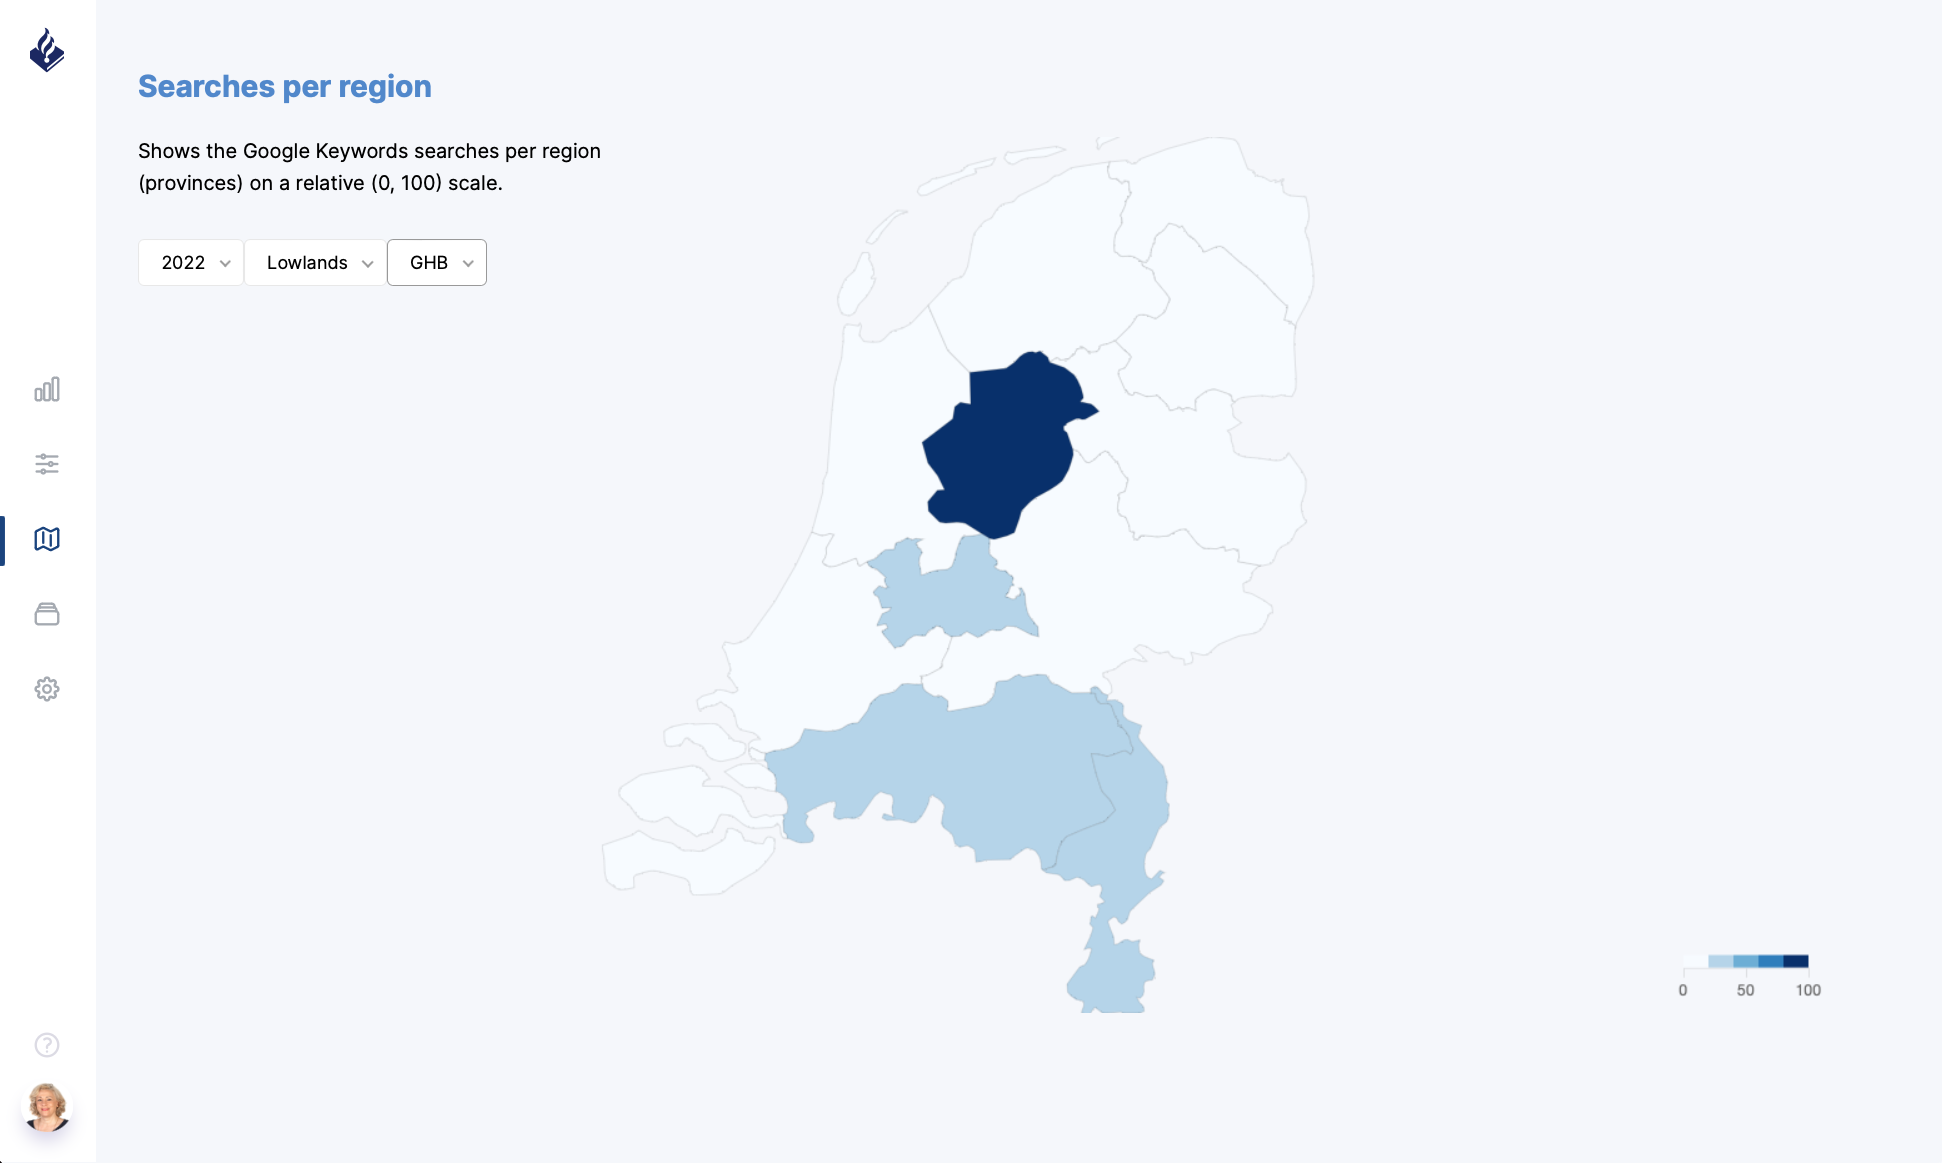
\includegraphics[width=\textwidth-2cm]{dashboard-2.png}
    \caption{Dashboard Prototype Region overview page with event Lowlands highlichted }
    \label{fig:event}
\end{figure*}

\subsection{Hosted source code}

As stated earlier, the source code of the web-based visualization, Python notebooks and datasets are hosted on GitHub using the MIT License. Under the \textit{uvadsp} username we have several code repositories:

\begin{enumerate}
  \item Notebooks: Source Code for the Jupyter Notebooks for data scraping and processing. \underline{https://github.com/uvadsp/notebooks}
  \item Visualization: Source Code for web application visualization dashboard. \underline{https://github.com/uvadsp/visualization}
  \item Datasets: The processed datasets in different formats to download. \underline{https://github.com/uvadsp/datasets}
\end{enumerate}

\subsection{Live version}
A live demo version of the web based visualization (desktop only) is hosted on Netlify and can be viewed using the following link \underline{https://uvadsp.netlify.app}

\subsection{Proportion test results}
The test results per drug per event and per data sources are presented below. 
\begin{enumerate}
    \item XTC
        \begin{figure*}[!htbp]
            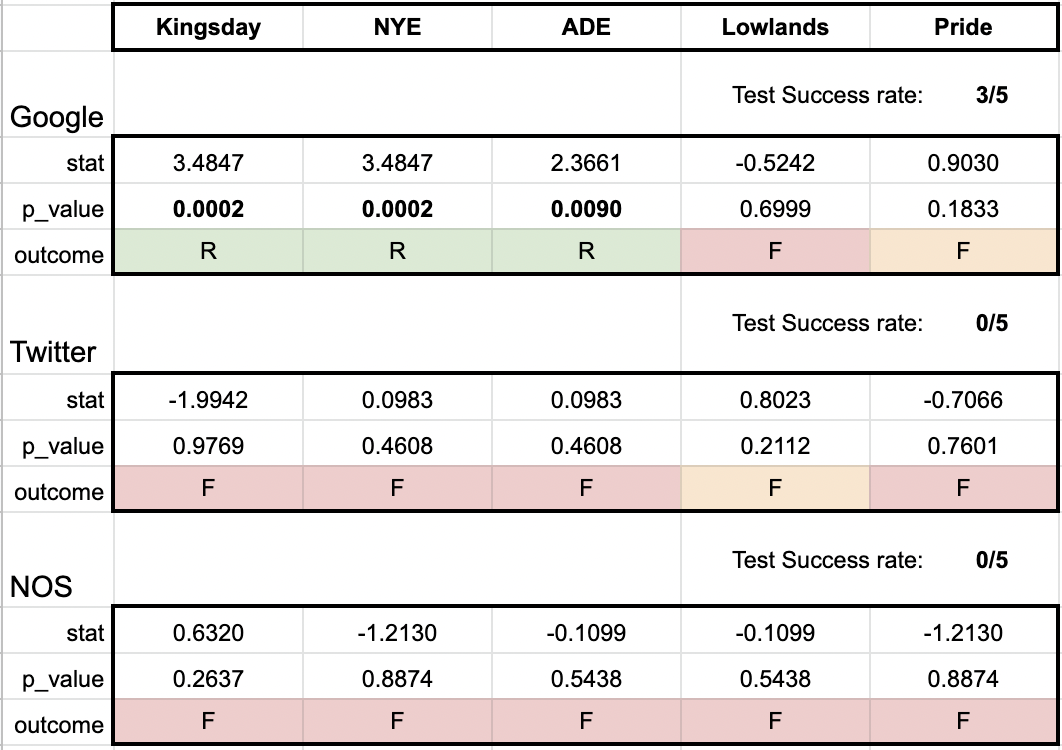
\includegraphics[width=3.25in]{XTC.png}
            \caption{Proportion test results per event and data source for XTC}
            \label{fig:XTC}
        \end{figure*}
    \item Cocaine
        \begin{figure*}[!htbp]
            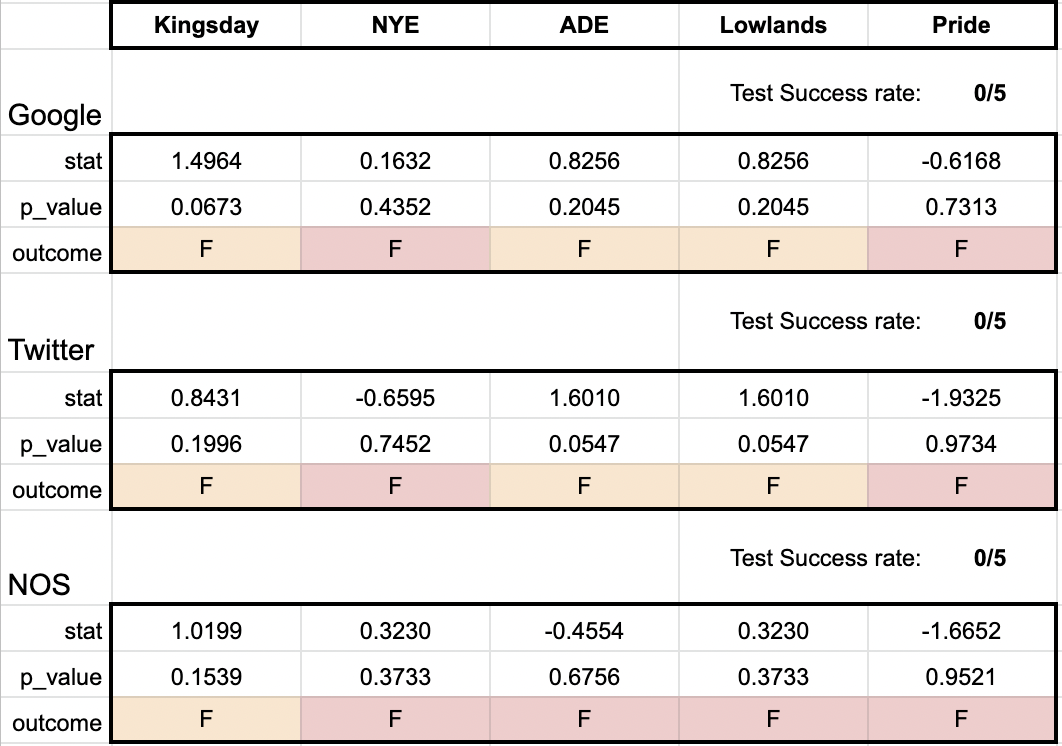
\includegraphics[width=3.25in]{Cocaine.png}
            \caption{Proportion test results per event and data source for Cocaine}
            \label{fig:Cocaine}
        \end{figure*}
    \item GHB
            \begin{figure*}[!htbp]
            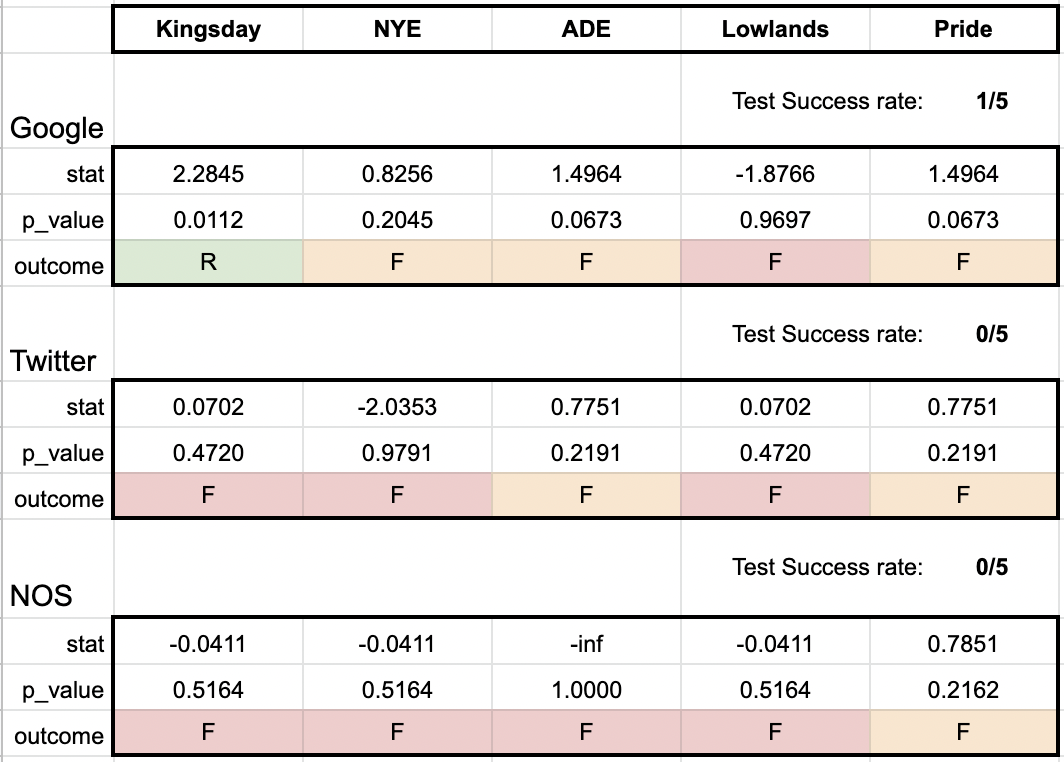
\includegraphics[width=3.25in]{GHB.png}
            \caption{Proportion test results per event and data source for GHB}
            \label{fig:Cocaine}
        \end{figure*}
\end{enumerate}

\subsection{Events}
Event dates over the years
\begin{figure*}[h]
    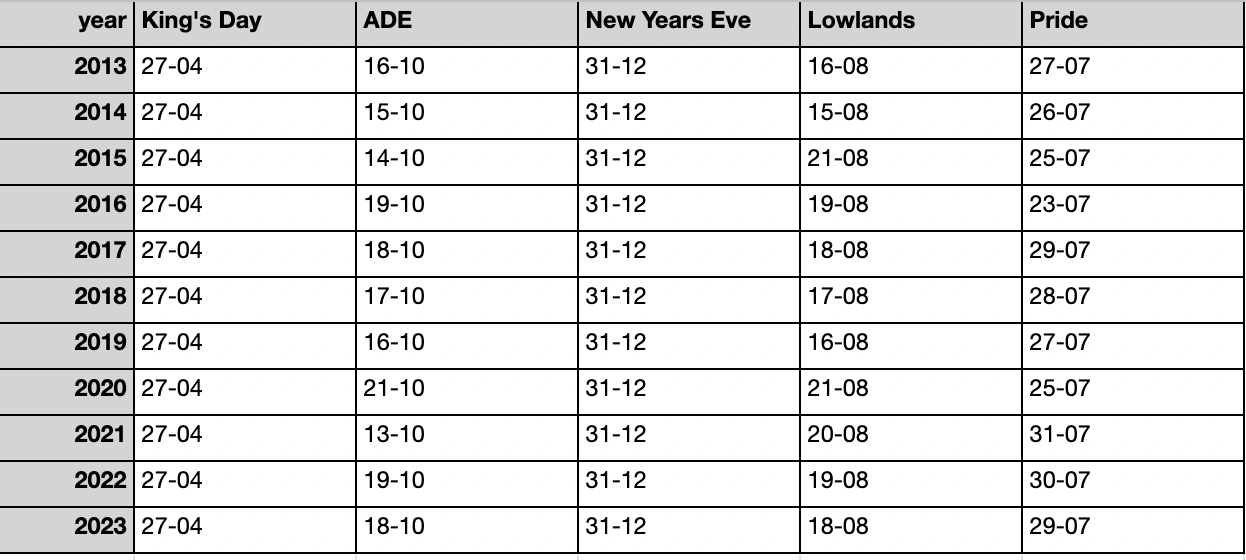
\includegraphics[width=3.25in]{event_dates.png}
    \caption{Event dates per year}
    \label{fig:event_dates}
\end{figure*}